\documentclass[11pt, a4paper]{article}
\usepackage[paper=a4paper, left=1.5cm, right=1.5cm, bottom=1.5cm, top=1.5cm]{geometry}
%
\usepackage[utf8]{inputenc}
\usepackage[spanish]{babel}

\usepackage{caratula/caratula}

\begin{document}

\titulo{Trabajo Práctico The Curry Game}
\fecha{25 de Mayo de 2016}
\materia{Ingeniería del Software II}

\integrante{Juan Carlos Giudici}{827/06}{elchudi@gmail.com}
\integrante{Andrés Navarro}{111/10}{roberto@gmail.com}
\integrante{Gonzalo Guillamon}{111/10}{roberto@gmail.com}
\integrante{Tomás Freilij}{111/10}{roberto@gmail.com}
%Carátula
\maketitle
\newpage

%Indice
\tableofcontents
\newpage

\section{Introducción}

El siguiente informe detallará el proceso que se siguió para resolver una problema definido siguiendo un esquema de trabajo con Scrum. Además se mencionarán problemas que se tuvieron en el transcurso del mismo y sus respectivas soluciones, así como la justificación de las decisiones tomadas.

Por último se procederá a exponer algunas conclusiones que sacamos de la experiencia con esta metodología.

\section{Aspectos de la metodología}

Como bien dijimos, vamos a utilizar Scrum para guiar el desarrollo del trabajo. En ese sentido, tuvimos las siguientes etapas:

\begin{itemize}

\item Armado de User Stories
\item Armado de un primer Sprint
\item Desarrollo del mismo
\item Review y armado del segundo Sprint
\item Cierre del trabajo

\end{itemize}

\section{Armado de User Stories}

Para este proceso lo que hicimos fue armar un conjunto de User Stories que, al resolverlas, consideremos como finalizado el trabajo.
En ese sentido, probablemente elegiríamos pocas stories pero muy generales y que por ende serían necesario subdividir en subitems.

Luego de esto definimos el esfuerzo y business value de cada una para poder armar el primer sprint.

Veamos detalles y decisiones de cada una de estas partes.

\subsection{Actores}

Las user stories que pensábamos íban dirigidas a dos tipos de actores:

\begin{itemize}

\item Diseñador de Juego (DJ): Representa al integrante del Stakeholder que modificará el comportamiento configurable de la aplicación. Por ejemplo, existe un cap inicial para cada participante, que en un futuro podría cambiar y que debería ser algo manipulable por este actor.

\item Participante : representa a la persona que usará la aplicación en producción.

\end{itemize}


\subsection{Asignación de esfuerzo}

El proceso fue recorrer las User Stories de comienzo a fin y en cada paso asignamos un valor, siempre comparando con los anteriores. 

Esto se contrapuso a la propuesta de la materia que planteaba leer todas primero, definir una que represente a la unidad de Esfuerzo y en base a eso se define el resto.

En algunos casos la forma en la que trabajamos nos obligó a volver hacia atrás a recalcular el valor de esfuerzo que habíamos asignado a algunas de las stories, en función de cosas que surgían de stories posteriores.


\section{Lenguaje de Programación}

Dadas las experiencias de los cuatro integrantes del equipo llegamos a dos posibles candidatos: Java y Ruby.

Luego de una discusión breve, nos quedamos con ruby principalmente porque preferimos desarrollar con lenguajes sin tipado estático por la flexibilidad que aporta en los modelos.  Ruby tiene la ventaja además de poder expresar ciertos patrones más fácilmente debido a la existencia de closures en el lenguaje.
\section{Desarrollo y modelado}

En esta sección presentaremos las decisiones de diseño que tomamos para desarrollar la aplicación. Para esto, explicaremos las entidades del problema y se adjuntan diagramas de objetos, de clases y de secuencia para clarificar.

\subsection{Una simulación}

Como bien sabemos, una simulación se ejecutará en el momento en que un Participante envíe un reto y otro se lo acepte.

En ese sentido, en el contexto de un duelo, el participante elegirá el equipo que lo represente. Un equipo conocerá cinco jugadores (base,ala,escolta,ala pivote y pivote), un director técnico y un nombre. 

Cada jugador conocerá un conjunto de estadísticas que afectarán su rendimiento en el partido.
Cada técnico conocerá un libro de estrategias en donde estarán las posibles jugadas que hará su equipo durante la simulación.


\begin{center}
\includegraphics[height=140px, width=300px]{img/DC-Equipo.png} 
\end{center}


De esta forma, en el contexto de una simulación, tenemos 

\begin{center}
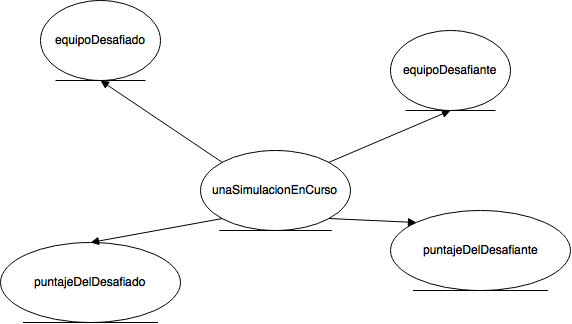
\includegraphics[height=140px, width=300px]{img/DO-SimulacionEnCurso.png} 
\end{center}


Una simulación tiene dos estados, en curso o terminada. Una en curso conoce el puntaje del desafiante y el desafiado, que luego cuando pase al estado de terminada, será el puntaje definitivo de la simulación.
Para modelar esto usamos el patrón State como muestra el siguiente diagrama de clases.

\begin{center}
\includegraphics[height=140px, width=300px]{img/DC-Simulacion.png}
\end{center}


Las posibles jugadas que pueden hacer los jugadores las modelamos con la idea de una Acción.

\section{Escenarios}

A continuación presentaremos algunos escenarios que nos parecieron interesantes como ejemplo para entender el modelo.

\subsection{Un pase con robo y contraofensiva exitosa}


\subsection{Un tiro con rebote y contraofensiva exitosa}

\section{Conclusiones}

El trabajo lo separamos en dos grandes momentos: Armado de Backlog e implementación del mismo.

Durantes las dos primeras semanas nos dedicamos a la primer parte, con dificultades para poder armar User Stories claras y correctamente definidas. En ese proceso consideramos que ciertas tareas ya las podíamos empezar a resolver. Sin embargo, respetando la metodología, no podíamos embarcarnos en esa tarea.

En ese sentido, nos parece que la metodología puede, por momentos, trabar el desarrollo del trabajo, convirtiéndose en una traba.


\end{document}
